\section{Encuestas}

Esta parte del sistema te permite conocer qué opinan tus clientes sobre el servicio de Perú Flores.
Ya tienes una encuesta lista llamada \textbf{``ENCUESTA DE SATISFACCIÓN DEL SERVICIO PERÚ FLORES''}, con 10 preguntas preparadas para que la uses cuando quieras.

% ─────────────────────────────────────────────────────────────────────────────
\subsection{Cómo ver tus encuestas}

Aquí puedes ver todas las encuestas que tiene el negocio. Desde esta pantalla puedes abrirlas,
compartirlas con tus clientes o revisar cuántas personas ya las respondieron.

\begin{figure}[H]
    \centering
    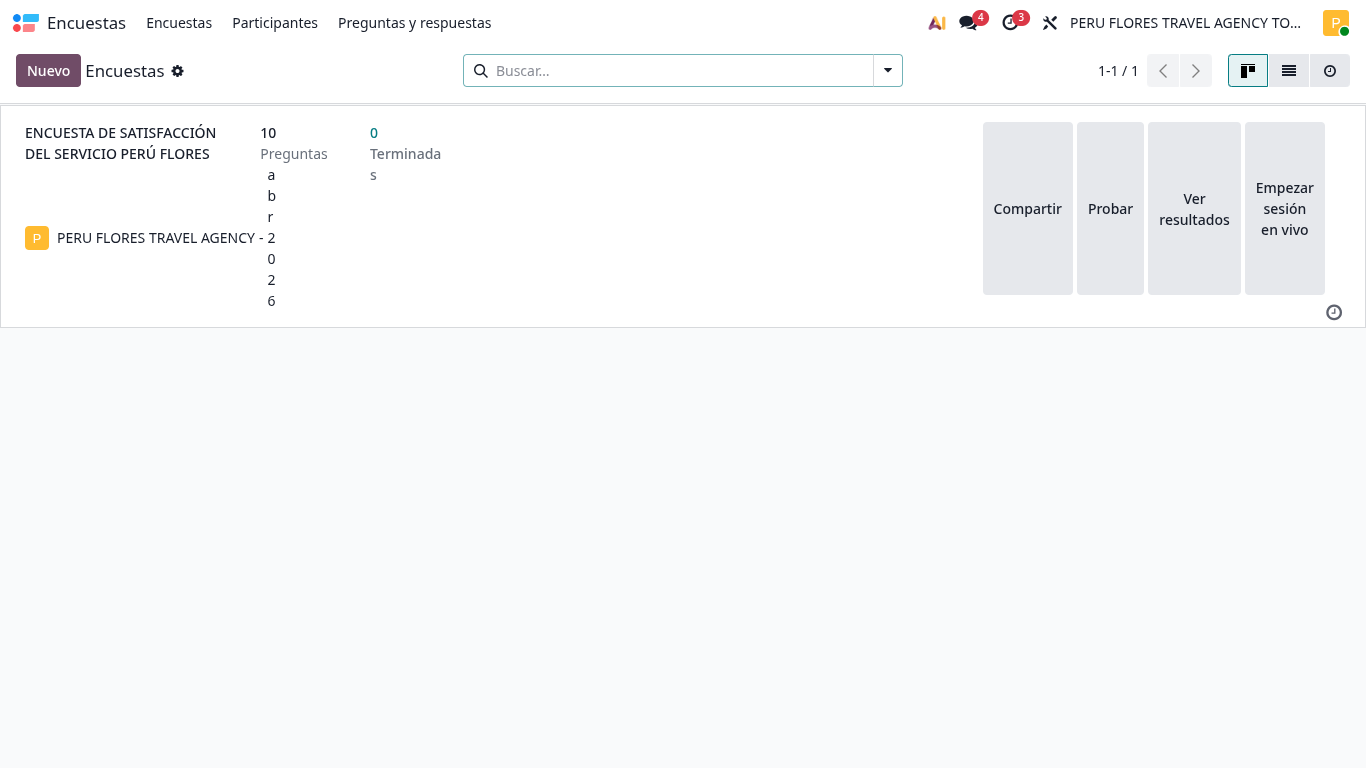
\includegraphics[width=0.9\textwidth]{assets/enc_01_lista.png}
    \caption{Pantalla principal de Encuestas --- tu encuesta de satisfacción aparece aquí}
\end{figure}

Desde esta pantalla puedes ver, en la misma fila de la encuesta, cuatro botones de acción rápida:

\begin{enumerate}
    \item El botón que dice \textbf{``Compartir''} te sirve para enviarles a tus clientes un enlace o un correo para que respondan la encuesta.
    \item El botón que dice \textbf{``Probar''} te abre la encuesta tal como la verían tus clientes, sin guardar nada. Úsalo para revisar que todo se vea bien antes de enviarla.
    \item El botón que dice \textbf{``Ver resultados''} te muestra un resumen con todas las respuestas que ya has recibido.
    \item El botón que dice \textbf{``Empezar sesión en vivo''} te permite proyectar la encuesta en tiempo real frente a un grupo, como si fuera una presentación.
\end{enumerate}

% ─────────────────────────────────────────────────────────────────────────────
\subsection{Cómo crear una encuesta nueva}

Si algún día necesitas armar una encuesta diferente, esto es todo lo que tienes que hacer.

\begin{figure}[H]
    \centering
    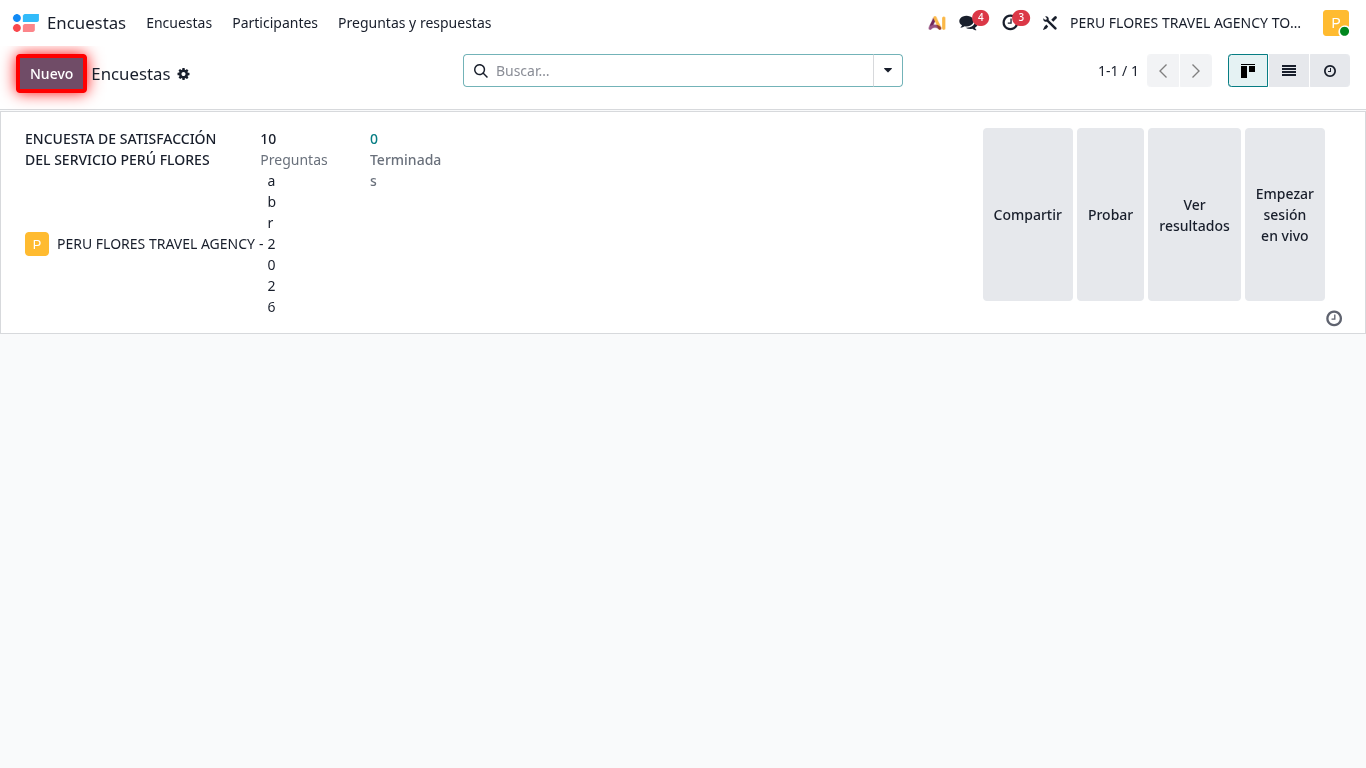
\includegraphics[width=0.9\textwidth]{assets/enc_02_nuevo_highlight.png}
    \caption{El botón \textbf{``Nuevo''} (marcado en rojo) para crear una encuesta desde cero}
\end{figure}

Sigue estos pasos:

\begin{enumerate}
    \item Busca en la parte de arriba, a la izquierda, el botón que dice \textbf{``Nuevo''} (lo hemos marcado con un cuadro rojo en la imagen de arriba para que sea fácil de encontrar).
    \item Haz clic ahí y se abrirá una pantalla en blanco lista para que llenes tu nueva encuesta.
\end{enumerate}

% ─────────────────────────────────────────────────────────────────────────────
\subsection{Cómo rellenar el formulario de una encuesta nueva}

Cuando abres una encuesta nueva (o la que ya existe), verás esta pantalla donde puedes ponerle
nombre a la encuesta y agregarle todas las preguntas que necesites.

\begin{figure}[H]
    \centering
    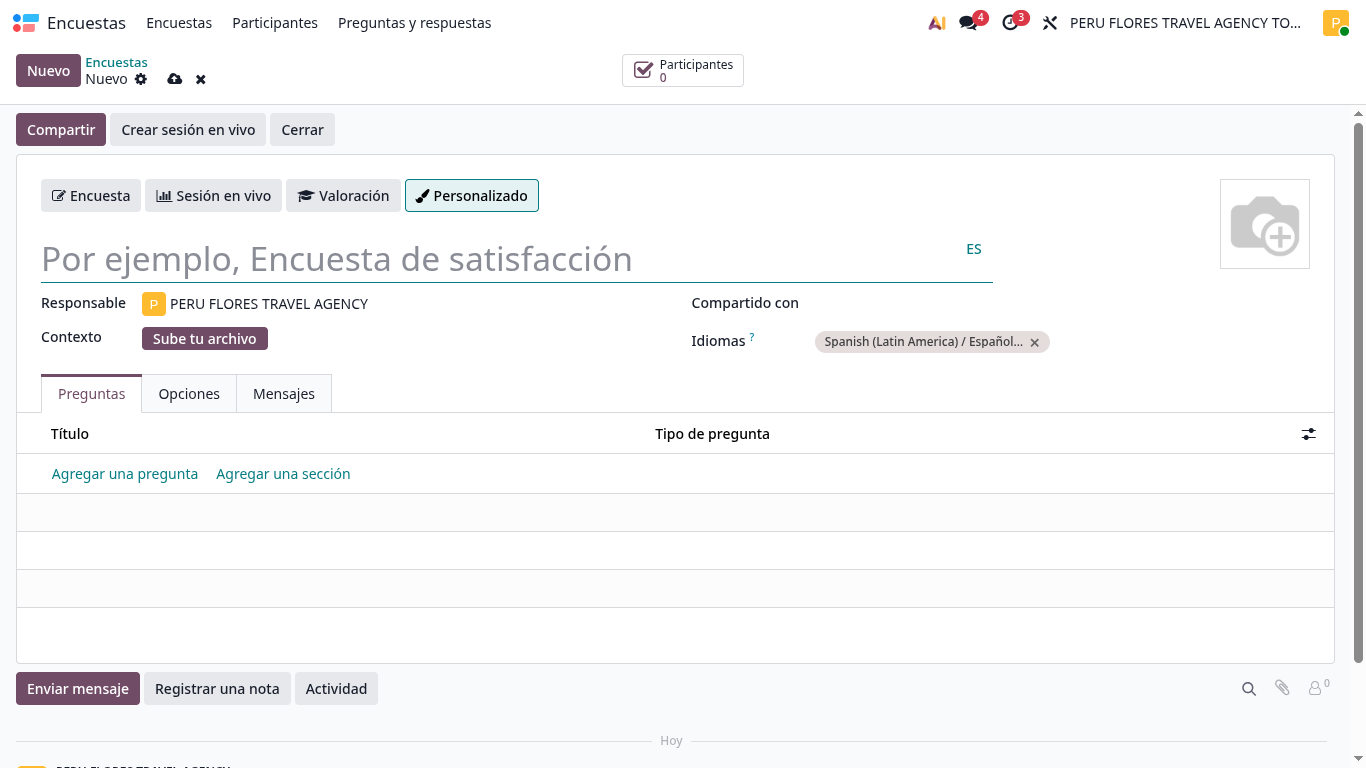
\includegraphics[width=0.9\textwidth]{assets/enc_03_formulario_encuesta.png}
    \caption{Pantalla para armar la encuesta: título, pestañas y área de preguntas}
\end{figure}

Esto es lo que ves en esa pantalla y para qué sirve cada cosa:

\begin{enumerate}
    \item En la parte de arriba donde dice \textbf{``Por ejemplo, Encuesta de satisfacción''} es donde escribes el nombre que le quieres poner a tu encuesta. Borra ese texto y escribe el tuyo.
    \item Debajo del nombre verás tres pestañas: \textbf{``Preguntas''}, \textbf{``Opciones''} y \textbf{``Mensajes''}. Empieza siempre por la pestaña \textbf{``Preguntas''}.
    \item En la pestaña \textbf{``Preguntas''} verás el área donde vas a agregar todas las preguntas de tu encuesta.
\end{enumerate}

% ─────────────────────────────────────────────────────────────────────────────
\subsection{Cómo agregar preguntas a la encuesta}

Una vez que le pusiste nombre a tu encuesta, es hora de agregar las preguntas que tus clientes van a responder.

\begin{figure}[H]
    \centering
    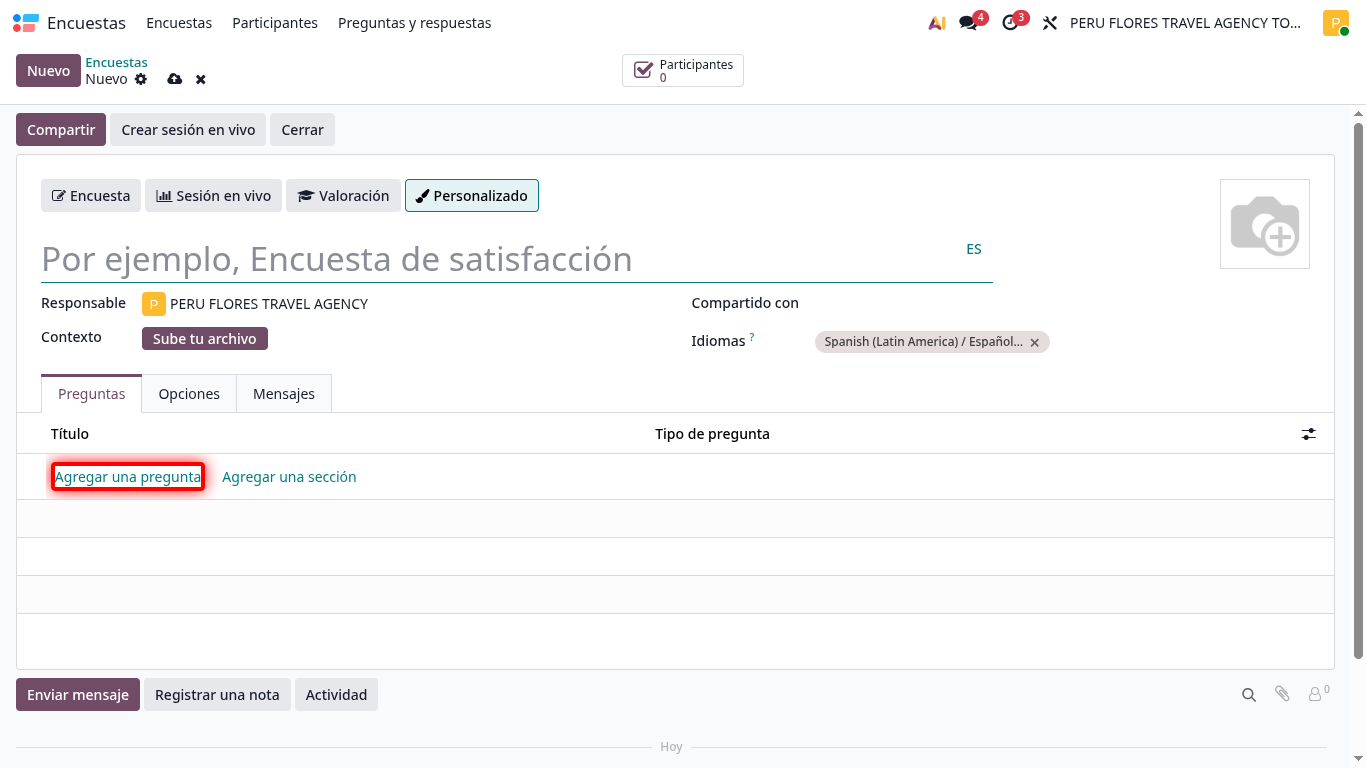
\includegraphics[width=0.9\textwidth]{assets/enc_05_agregar_pregunta_highlight.png}
    \caption{El enlace \textbf{``Agregar una pregunta''} (marcado en rojo) dentro de la pestaña \textbf{``Preguntas''}}
\end{figure}

Sigue estos pasos:

\begin{enumerate}
    \item Asegúrate de estar en la pestaña que dice \textbf{``Preguntas''}.
    \item Busca el texto que dice \textbf{``Agregar una pregunta''} (lo hemos marcado con un cuadro rojo en la imagen de arriba).
    \item Haz clic ahí. Se abrirá una ventanita donde puedes escribir tu pregunta y elegir qué tipo de respuesta quieres (por ejemplo, varias opciones para elegir, un número del 1 al 5, o un cuadro para escribir libremente).
    \item Una vez que termines de escribir la pregunta, haz clic en el botón que dice \textbf{``Guardar y cerrar''} para que quede registrada.
    \item Repite este proceso para cada pregunta que quieras agregar.
    \item Cuando hayas puesto todas las preguntas, haz clic en el botón que dice \textbf{``Guardar''} (está en la barra de arriba, con un ícono de nube) para no perder los cambios.
\end{enumerate}

\bigskip
\noindent\textbf{Nota:} Si necesitas dividir la encuesta en partes (por ejemplo, primero preguntas sobre el precio, luego sobre la atención), puedes usar el enlace que dice \textbf{``Agregar una sección''} que está justo al lado.

% ─────────────────────────────────────────────────────────────────────────────
\subsection{Cómo enviar la encuesta a tus clientes}

Cuando tu encuesta ya está lista y guardada, puedes enviarla. Esto es lo más importante: que tus clientes la reciban y la respondan.

\begin{figure}[H]
    \centering
    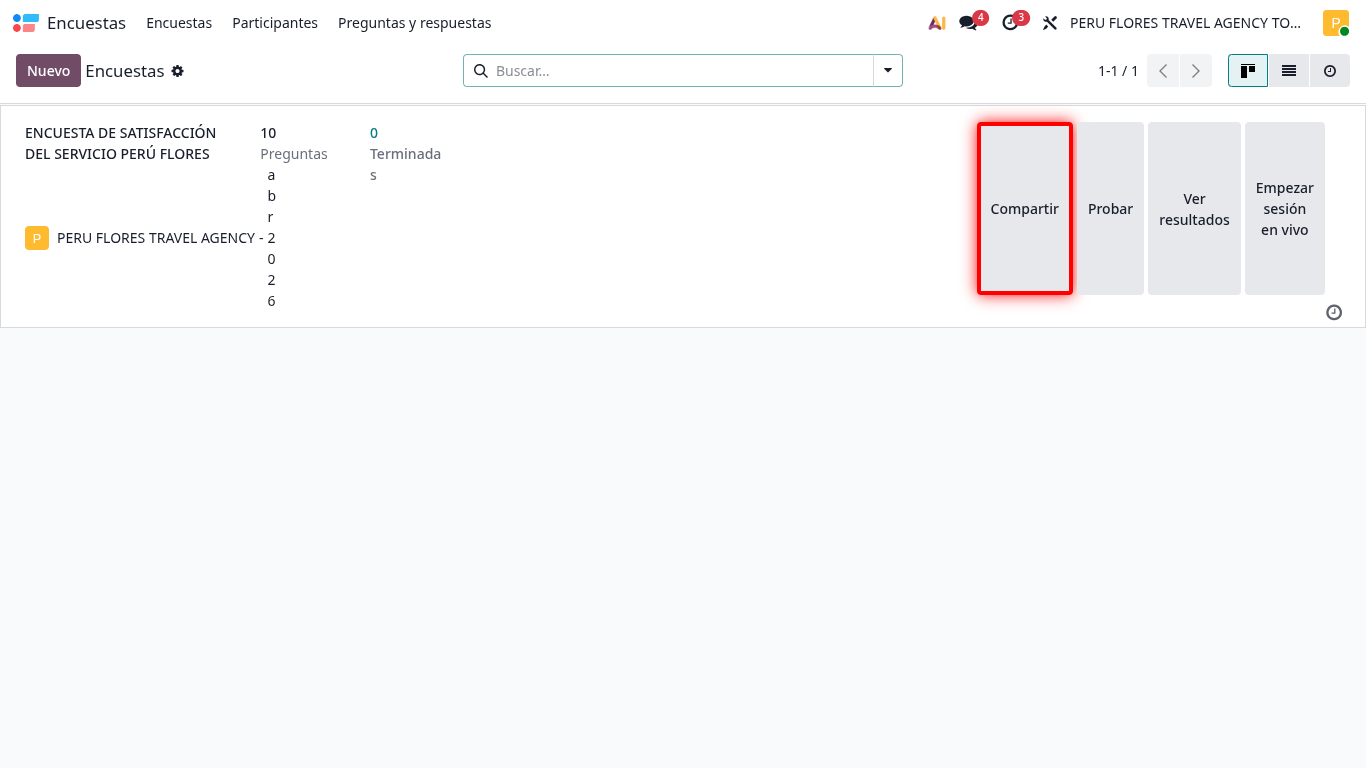
\includegraphics[width=0.9\textwidth]{assets/enc_14_compartir_highlight.png}
    \caption{El botón \textbf{``Compartir''} (marcado en rojo) en la fila de tu encuesta}
\end{figure}

Sigue estos pasos:

\begin{enumerate}
    \item Desde la pantalla principal de Encuestas, busca tu encuesta en la lista.
    \item En la misma fila de tu encuesta, haz clic en el botón que dice \textbf{``Compartir''} (lo hemos marcado con un cuadro rojo en la imagen de arriba).
    \item Se abrirá una pequeña ventana como la que ves a continuación:
\end{enumerate}

\begin{figure}[H]
    \centering
    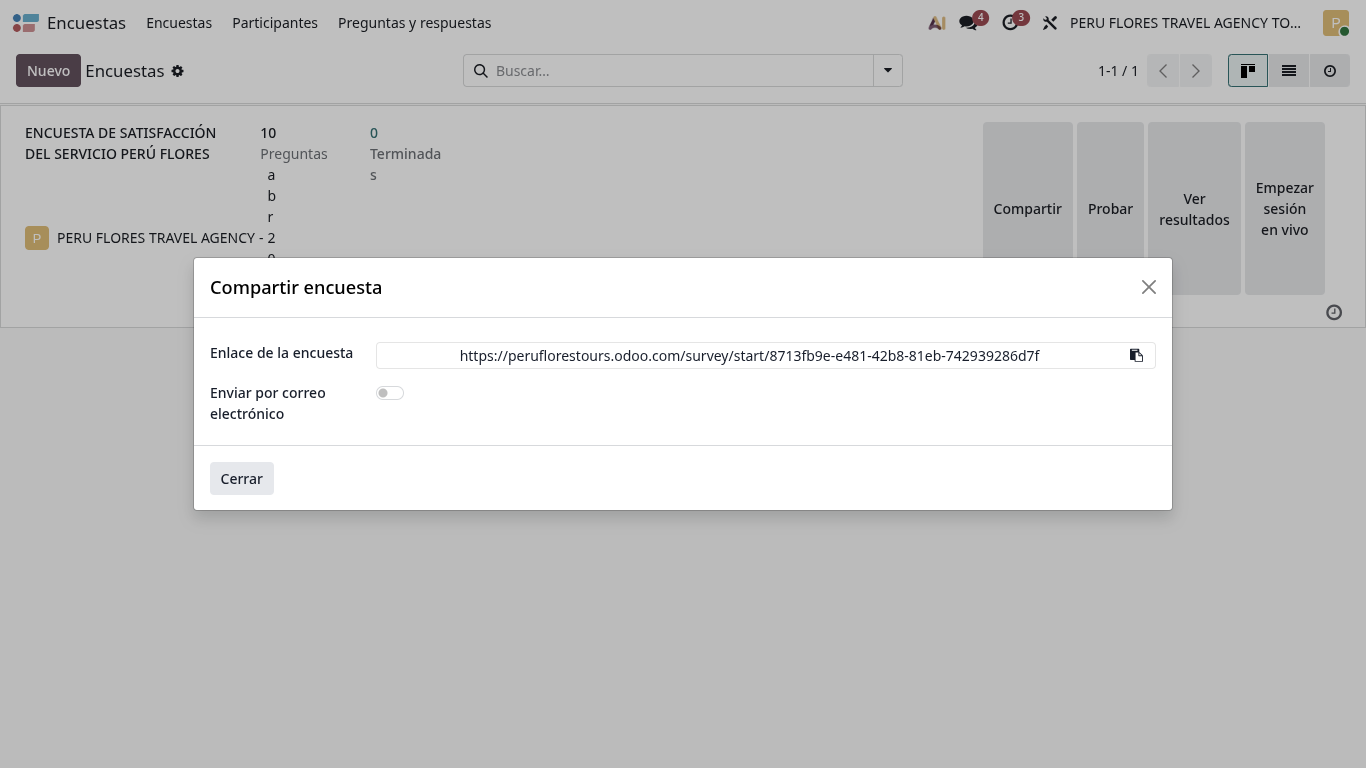
\includegraphics[width=0.85\textwidth]{assets/enc_15_pantalla_compartir.png}
    \caption{Ventana \textbf{``Compartir encuesta''} con el enlace listo para copiar y la opción de envío por correo}
\end{figure}

\begin{enumerate}
    \setcounter{enumi}{3}
    \item En esa ventana verás dos cosas:
    \begin{itemize}
        \item \textbf{Enlace de la encuesta:} es un link que puedes copiar haciendo clic en el ícono de copiar que está al lado. Luego pégalo en WhatsApp, en un correo o en tus redes sociales para que tus clientes lo abran.
        \item \textbf{Enviar por correo electrónico:} si activas esa opción (el interruptor que dice \textbf{``Enviar por correo electrónico''}), podrás escribir los correos de tus clientes directamente y el sistema les enviará el enlace automáticamente.
    \end{itemize}
    \item Cuando termines, haz clic en el botón que dice \textbf{``Cerrar''} para salir de esa ventana.
\end{enumerate}

% ─────────────────────────────────────────────────────────────────────────────
\subsection{Cómo ver cuántos respondieron y qué dijeron}

Una vez que tus clientes empiecen a contestar, puedes revisar los resultados en cualquier momento.

\begin{figure}[H]
    \centering
    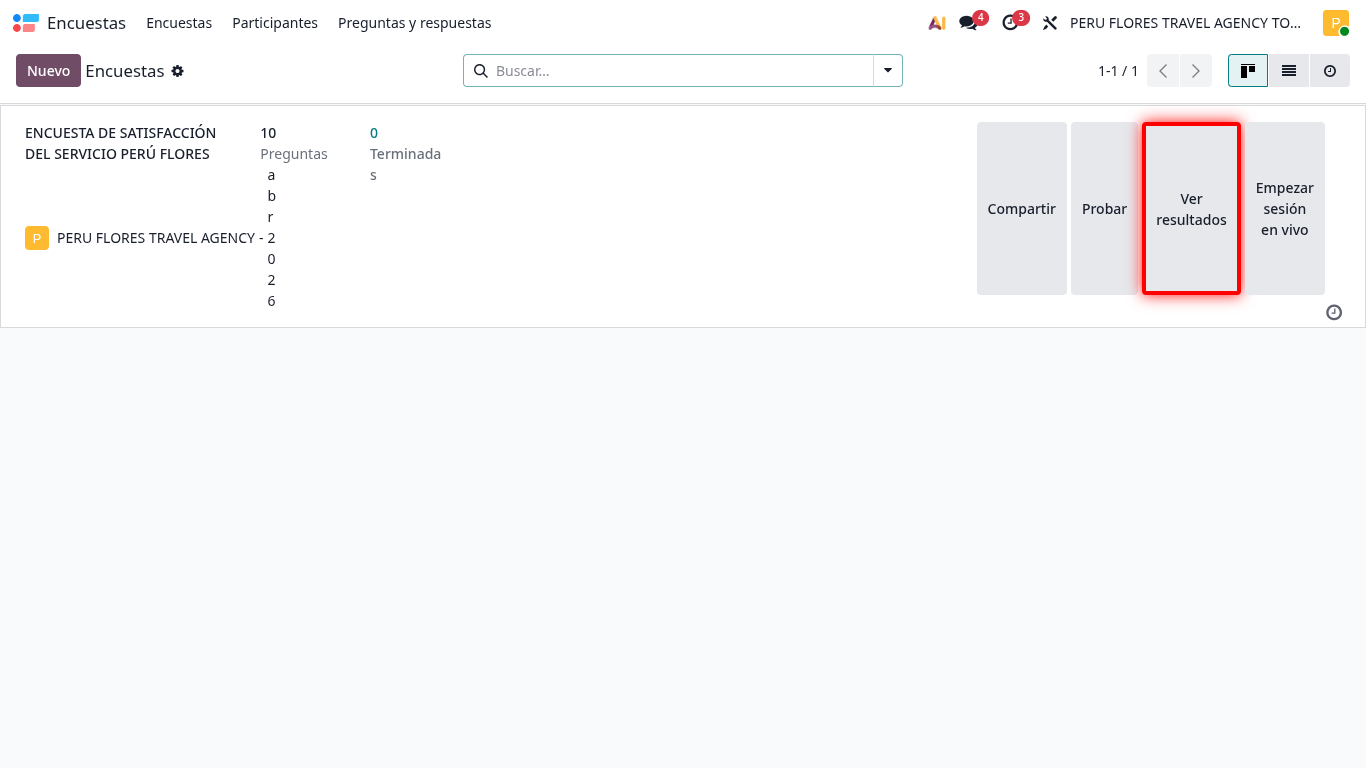
\includegraphics[width=0.9\textwidth]{assets/enc_18_ver_resultados_highlight.png}
    \caption{El botón \textbf{``Ver resultados''} (marcado en rojo) que te lleva al resumen de respuestas}
\end{figure}

Sigue estos pasos:

\begin{enumerate}
    \item Desde la pantalla principal de Encuestas, busca tu encuesta en la lista.
    \item Fíjate en el número que aparece debajo de \textbf{``Terminadas''}: ese número te dice cuántas personas ya la respondieron completamente.
    \item Haz clic en el botón que dice \textbf{``Ver resultados''} en la fila de tu encuesta (lo hemos marcado con un cuadro rojo en la imagen de arriba).
    \item Se abrirá una pantalla con un resumen de todas las respuestas que han llegado. Cuando haya respuestas, podrás ver gráficas con los resultados de cada pregunta.
    \item Usa esa información para mejorar el servicio de Perú Flores según lo que opinaron tus clientes.
\end{enumerate}

\bigskip
\noindent\textbf{Recuerda:} La encuesta \textbf{``ENCUESTA DE SATISFACCIÓN DEL SERVICIO PERÚ FLORES''} ya está lista para usar.
Solo tienes que hacer clic en \textbf{``Compartir''} y enviarla después de cada tour o servicio para conocer la experiencia de tus clientes.
